\section{Simulation Analysis}
\label{sec:simulation}

\subsection{Operating Point Analysis}

Table~\ref{tab:op} shows the simulated operating point results for the circuit
under analysis. Compared to the theoretical analysis results, one notices the
following differences: describe and explain the differences.


\begin{figure}[h] \centering
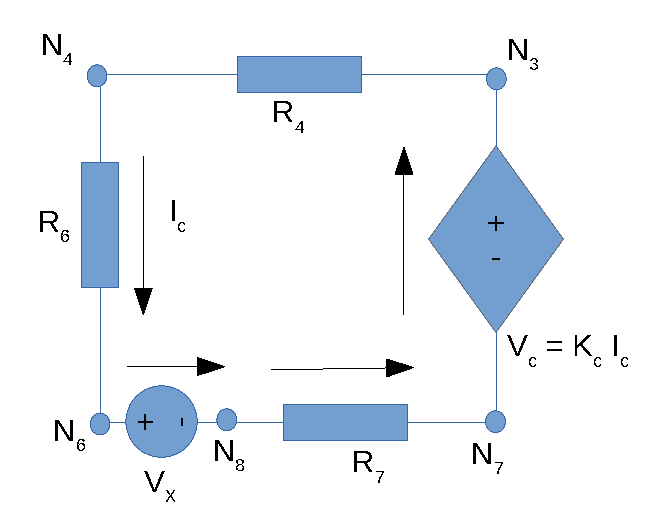
\includegraphics[width=0.4\linewidth]{malhaC.pdf}
\caption{C Mesh with an adicional voltage source} %mudar legendaaaaaaaaaaa!!!!!!
\label{fig:malhaC}
\end{figure}

The table below shows the simulated operating point results for the circuit described in Figure 1.

In this simulation is important to explain the creation of a auxiliary voltage Vb (with voltage equal to 0V) that was put between N6 and R7. Consequently this led to appearance of a node that we designated by N8 that has the same voltage as N6.

This was necessary because of Ngspice software requirements.

By observing the table we can conclude that the simulated results are the same of the theoretical results.

\begin{table}[h]
  \centering
  \begin{tabular}{|l|r|}
    \hline    
    {\bf Name} & {\bf Value [A or V]} \\ \hline
    @cb[i] & 0.000000e+00\\ \hline
@ce[i] & 0.000000e+00\\ \hline
@q1[ib] & 7.022567e-05\\ \hline
@q1[ic] & 1.404513e-02\\ \hline
@q1[ie] & -1.41154e-02\\ \hline
@q1[is] & 5.765392e-12\\ \hline
@rc[i] & 1.411536e-02\\ \hline
@re[i] & 1.411536e-02\\ \hline
@rf[i] & 7.022567e-05\\ \hline
@rs[i] & 0.000000e+00\\ \hline
v(1) & 0.000000e+00\\ \hline
v(2) & 0.000000e+00\\ \hline
base & 2.254108e+00\\ \hline
coll & 5.765392e+00\\ \hline
emit & 1.411536e+00\\ \hline
vcc & 1.000000e+01\\ \hline

  \end{tabular}
  \caption{Operating point. A variable preceded by @ is of type {\em current}
    and expressed in Ampere; other variables are of type {\it voltage} and expressed in
    Volt.}
  \label{tab:op}
\end{table}




